% ================= Phase 4 新增內容 =================
% 標示「待補」的地方需要實作 session 的最終 SQL、示範資料或系統畫面，不可自行編造。
\newcommand{\todo}[1]{\par\noindent\fbox{\parbox{0.95\linewidth}{\small\textbf{待補：}#1}}\par\medskip}
\newcommand{\resultimg}[2]{% {檔名}{說明}
\IfFileExists{img/#1}{\begin{center}\includegraphics[width=0.95\linewidth]{img/#1}\\[-0.3em]{\small #2}\end{center}}{\todo{#2（\texttt{\detokenize{img/#1}}）}}}

% ================= Section 5 =================
\clearpage
\section{函數相依與資料庫正規化 (Functional Dependencies and Database Normalization)}

\subsection{函數相依 (Functional Dependencies)}

以下依 Section 4 的 16 張資料表（Phase 3 實作版本）列出每張表的非平凡函數相依。每張圖上方為資料表的屬性，底線為主鍵；下方每條橫線代表一條 FD：粗線連到的屬性是決定者，箭頭指向被決定的屬性；同一張表有多條 FD 時，各條 FD 的直線左右稍微錯開。只有主鍵、沒有其他屬性的表（如 \at{USER_ROLE}）沒有非平凡 FD。

\par\noindent\begin{adjustbox}{max width=\linewidth}
\begin{tikzpicture}[font=\scriptsize\ttfamily, box/.style={draw,minimum height=0.55cm,inner sep=2pt,anchor=west}]
\node[anchor=south west,font=\small\bfseries\sffamily] at (0,0.32) {USERS};
\node[box,minimum width=1.33cm] at (0.00,0) {\underline{user\_id}};
\node[box,minimum width=1.33cm] at (1.33,0) {loginid};
\node[box,minimum width=0.90cm] at (2.67,0) {name};
\node[box,minimum width=2.27cm] at (3.57,0) {password\_hash};
\node[box,minimum width=1.02cm] at (5.83,0) {email};
\node[box,minimum width=1.33cm] at (6.86,0) {address};
\node[box,minimum width=1.02cm] at (8.20,0) {phone};
\node[box,minimum width=1.65cm] at (9.22,0) {is\_active};
\node[box,minimum width=1.80cm] at (10.87,0) {created\_at};
\node[anchor=east,font=\scriptsize\sffamily\bfseries] at (-0.05,-0.79) {FD1};
\draw (0.59,-0.79) -- (11.69,-0.79);
\draw[line width=1.1pt] (0.59,-0.28) -- (0.59,-0.79);
\draw[-{Stealth[length=4pt]}] (1.92,-0.79) -- (1.92,-0.28);
\draw[-{Stealth[length=4pt]}] (3.04,-0.79) -- (3.04,-0.28);
\draw[-{Stealth[length=4pt]}] (4.62,-0.79) -- (4.62,-0.28);
\draw[-{Stealth[length=4pt]}] (6.27,-0.79) -- (6.27,-0.28);
\draw[-{Stealth[length=4pt]}] (7.45,-0.79) -- (7.45,-0.28);
\draw[-{Stealth[length=4pt]}] (8.63,-0.79) -- (8.63,-0.28);
\draw[-{Stealth[length=4pt]}] (9.96,-0.79) -- (9.96,-0.28);
\draw[-{Stealth[length=4pt]}] (11.69,-0.79) -- (11.69,-0.28);
\node[anchor=east,font=\scriptsize\sffamily\bfseries] at (-0.05,-1.13) {FD2};
\draw (0.75,-1.13) -- (11.85,-1.13);
\draw[line width=1.1pt] (2.08,-0.28) -- (2.08,-1.13);
\draw[-{Stealth[length=4pt]}] (0.75,-1.13) -- (0.75,-0.28);
\draw[-{Stealth[length=4pt]}] (3.20,-1.13) -- (3.20,-0.28);
\draw[-{Stealth[length=4pt]}] (4.78,-1.13) -- (4.78,-0.28);
\draw[-{Stealth[length=4pt]}] (6.43,-1.13) -- (6.43,-0.28);
\draw[-{Stealth[length=4pt]}] (7.61,-1.13) -- (7.61,-0.28);
\draw[-{Stealth[length=4pt]}] (8.79,-1.13) -- (8.79,-0.28);
\draw[-{Stealth[length=4pt]}] (10.12,-1.13) -- (10.12,-0.28);
\draw[-{Stealth[length=4pt]}] (11.85,-1.13) -- (11.85,-0.28);
\end{tikzpicture}
\end{adjustbox}\par\medskip

\par\noindent\begin{adjustbox}{max width=\linewidth}
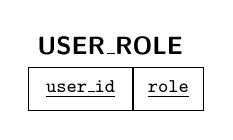
\begin{tikzpicture}[font=\scriptsize\ttfamily, box/.style={draw,minimum height=0.55cm,inner sep=2pt,anchor=west}]
\node[anchor=south west,font=\small\bfseries\sffamily] at (0,0.32) {USER\_ROLE};
\node[box,minimum width=1.33cm] at (0.00,0) {\underline{user\_id}};
\node[box,minimum width=0.90cm] at (1.33,0) {\underline{role}};
\end{tikzpicture}
\end{adjustbox}\par\medskip

\par\noindent\begin{adjustbox}{max width=\linewidth}
\begin{tikzpicture}[font=\scriptsize\ttfamily, box/.style={draw,minimum height=0.55cm,inner sep=2pt,anchor=west}]
\node[anchor=south west,font=\small\bfseries\sffamily] at (0,0.32) {STORE};
\node[box,minimum width=1.49cm] at (0.00,0) {\underline{store\_id}};
\node[box,minimum width=0.90cm] at (1.49,0) {name};
\node[box,minimum width=1.33cm] at (2.39,0) {address};
\node[box,minimum width=1.02cm] at (3.73,0) {email};
\node[box,minimum width=1.02cm] at (4.75,0) {phone};
\node[anchor=east,font=\scriptsize\sffamily\bfseries] at (-0.05,-0.79) {FD1};
\draw (0.74,-0.79) -- (5.26,-0.79);
\draw[line width=1.1pt] (0.74,-0.28) -- (0.74,-0.79);
\draw[-{Stealth[length=4pt]}] (1.94,-0.79) -- (1.94,-0.28);
\draw[-{Stealth[length=4pt]}] (3.06,-0.79) -- (3.06,-0.28);
\draw[-{Stealth[length=4pt]}] (4.24,-0.79) -- (4.24,-0.28);
\draw[-{Stealth[length=4pt]}] (5.26,-0.79) -- (5.26,-0.28);
\end{tikzpicture}
\end{adjustbox}\par\medskip

\par\noindent\begin{adjustbox}{max width=\linewidth}
\begin{tikzpicture}[font=\scriptsize\ttfamily, box/.style={draw,minimum height=0.55cm,inner sep=2pt,anchor=west}]
\node[anchor=south west,font=\small\bfseries\sffamily] at (0,0.32) {STORE\_STAFF};
\node[box,minimum width=1.33cm] at (0.00,0) {\underline{user\_id}};
\node[box,minimum width=1.49cm] at (1.33,0) {store\_id};
\node[anchor=east,font=\scriptsize\sffamily\bfseries] at (-0.05,-0.79) {FD1};
\draw (0.67,-0.79) -- (2.08,-0.79);
\draw[line width=1.1pt] (0.67,-0.28) -- (0.67,-0.79);
\draw[-{Stealth[length=4pt]}] (2.08,-0.79) -- (2.08,-0.28);
\end{tikzpicture}
\end{adjustbox}\par\medskip

\par\noindent\begin{adjustbox}{max width=\linewidth}
\begin{tikzpicture}[font=\scriptsize\ttfamily, box/.style={draw,minimum height=0.55cm,inner sep=2pt,anchor=west}]
\node[anchor=south west,font=\small\bfseries\sffamily] at (0,0.32) {PRODUCT};
\node[box,minimum width=1.80cm] at (0.00,0) {\underline{product\_id}};
\node[box,minimum width=1.49cm] at (1.80,0) {store\_id};
\node[box,minimum width=0.90cm] at (3.29,0) {name};
\node[box,minimum width=1.96cm] at (4.19,0) {description};
\node[box,minimum width=1.49cm] at (6.15,0) {category};
\node[box,minimum width=1.65cm] at (7.64,0) {image\_url};
\node[box,minimum width=1.02cm] at (9.28,0) {price};
\node[box,minimum width=1.02cm] at (10.31,0) {stock};
\node[box,minimum width=1.65cm] at (11.33,0) {is\_listed};
\node[box,minimum width=1.80cm] at (12.98,0) {created\_at};
\node[box,minimum width=1.80cm] at (14.78,0) {updated\_at};
\node[anchor=east,font=\scriptsize\sffamily\bfseries] at (-0.05,-0.79) {FD1};
\draw (0.90,-0.79) -- (15.68,-0.79);
\draw[line width=1.1pt] (0.90,-0.28) -- (0.90,-0.79);
\draw[-{Stealth[length=4pt]}] (2.54,-0.79) -- (2.54,-0.28);
\draw[-{Stealth[length=4pt]}] (3.74,-0.79) -- (3.74,-0.28);
\draw[-{Stealth[length=4pt]}] (5.17,-0.79) -- (5.17,-0.28);
\draw[-{Stealth[length=4pt]}] (6.89,-0.79) -- (6.89,-0.28);
\draw[-{Stealth[length=4pt]}] (8.46,-0.79) -- (8.46,-0.28);
\draw[-{Stealth[length=4pt]}] (9.79,-0.79) -- (9.79,-0.28);
\draw[-{Stealth[length=4pt]}] (10.82,-0.79) -- (10.82,-0.28);
\draw[-{Stealth[length=4pt]}] (12.15,-0.79) -- (12.15,-0.28);
\draw[-{Stealth[length=4pt]}] (13.88,-0.79) -- (13.88,-0.28);
\draw[-{Stealth[length=4pt]}] (15.68,-0.79) -- (15.68,-0.28);
\end{tikzpicture}
\end{adjustbox}\par\medskip

\par\noindent\begin{adjustbox}{max width=\linewidth}
\begin{tikzpicture}[font=\scriptsize\ttfamily, box/.style={draw,minimum height=0.55cm,inner sep=2pt,anchor=west}]
\node[anchor=south west,font=\small\bfseries\sffamily] at (0,0.32) {CART\_ITEM};
\node[box,minimum width=1.33cm] at (0.00,0) {\underline{user\_id}};
\node[box,minimum width=1.80cm] at (1.33,0) {\underline{product\_id}};
\node[box,minimum width=1.49cm] at (3.13,0) {quantity};
\node[box,minimum width=1.49cm] at (4.62,0) {added\_at};
\node[anchor=east,font=\scriptsize\sffamily\bfseries] at (-0.05,-0.79) {FD1};
\draw (0.67,-0.79) -- (5.37,-0.79);
\draw[line width=1.1pt] (0.67,-0.28) -- (0.67,-0.79);
\draw[line width=1.1pt] (2.23,-0.28) -- (2.23,-0.79);
\draw[-{Stealth[length=4pt]}] (3.88,-0.79) -- (3.88,-0.28);
\draw[-{Stealth[length=4pt]}] (5.37,-0.79) -- (5.37,-0.28);
\end{tikzpicture}
\end{adjustbox}\par\medskip

\par\noindent\begin{adjustbox}{max width=\linewidth}
\begin{tikzpicture}[font=\scriptsize\ttfamily, box/.style={draw,minimum height=0.55cm,inner sep=2pt,anchor=west}]
\node[anchor=south west,font=\small\bfseries\sffamily] at (0,0.32) {ORDERS};
\node[box,minimum width=1.49cm] at (0.00,0) {\underline{order\_id}};
\node[box,minimum width=1.33cm] at (1.49,0) {user\_id};
\node[box,minimum width=1.80cm] at (2.83,0) {order\_time};
\node[box,minimum width=2.42cm] at (4.62,0) {recipient\_name};
\node[box,minimum width=2.58cm] at (7.04,0) {recipient\_phone};
\node[box,minimum width=2.88cm] at (9.62,0) {recipient\_address};
\node[box,minimum width=1.49cm] at (12.51,0) {subtotal};
\node[box,minimum width=2.42cm] at (14.00,0) {discount\_total};
\node[box,minimum width=0.90cm] at (16.41,0) {tax};
\node[box,minimum width=2.11cm] at (17.31,0) {shipping\_fee};
\node[box,minimum width=1.02cm] at (19.42,0) {total};
\node[box,minimum width=1.18cm] at (20.45,0) {status};
\node[box,minimum width=1.33cm] at (21.63,0) {paid\_at};
\node[anchor=east,font=\scriptsize\sffamily\bfseries] at (-0.05,-0.79) {FD1};
\draw (0.67,-0.79) -- (22.22,-0.79);
\draw[line width=1.1pt] (0.67,-0.28) -- (0.67,-0.79);
\draw[-{Stealth[length=4pt]}] (2.08,-0.79) -- (2.08,-0.28);
\draw[-{Stealth[length=4pt]}] (3.65,-0.79) -- (3.65,-0.28);
\draw[-{Stealth[length=4pt]}] (5.75,-0.79) -- (5.75,-0.28);
\draw[-{Stealth[length=4pt]}] (8.25,-0.79) -- (8.25,-0.28);
\draw[-{Stealth[length=4pt]}] (10.98,-0.79) -- (10.98,-0.28);
\draw[-{Stealth[length=4pt]}] (13.17,-0.79) -- (13.17,-0.28);
\draw[-{Stealth[length=4pt]}] (15.13,-0.79) -- (15.13,-0.28);
\draw[-{Stealth[length=4pt]}] (16.79,-0.79) -- (16.79,-0.28);
\draw[-{Stealth[length=4pt]}] (18.29,-0.79) -- (18.29,-0.28);
\draw[-{Stealth[length=4pt]}] (19.86,-0.79) -- (19.86,-0.28);
\draw[-{Stealth[length=4pt]}] (20.96,-0.79) -- (20.96,-0.28);
\draw[-{Stealth[length=4pt]}] (22.22,-0.79) -- (22.22,-0.28);
\node[anchor=east,font=\scriptsize\sffamily\bfseries] at (-0.05,-1.13) {FD2};
\draw (13.33,-1.13) -- (20.02,-1.13);
\draw[line width=1.1pt] (13.33,-0.28) -- (13.33,-1.13);
\draw[line width=1.1pt] (15.29,-0.28) -- (15.29,-1.13);
\draw[line width=1.1pt] (16.94,-0.28) -- (16.94,-1.13);
\draw[line width=1.1pt] (18.45,-0.28) -- (18.45,-1.13);
\draw[-{Stealth[length=4pt]}] (20.02,-1.13) -- (20.02,-0.28);
\end{tikzpicture}
\end{adjustbox}\par\medskip

\par\noindent\begin{adjustbox}{max width=\linewidth}
\begin{tikzpicture}[font=\scriptsize\ttfamily, box/.style={draw,minimum height=0.55cm,inner sep=2pt,anchor=west}]
\node[anchor=south west,font=\small\bfseries\sffamily] at (0,0.32) {ORDER\_ITEM};
\node[box,minimum width=1.49cm] at (0.00,0) {\underline{order\_id}};
\node[box,minimum width=1.33cm] at (1.49,0) {\underline{item\_no}};
\node[box,minimum width=1.80cm] at (2.83,0) {product\_id};
\node[box,minimum width=2.11cm] at (4.62,0) {product\_name};
\node[box,minimum width=1.80cm] at (6.73,0) {unit\_price};
\node[box,minimum width=1.49cm] at (8.54,0) {quantity};
\node[box,minimum width=2.42cm] at (10.03,0) {event\_discount};
\node[anchor=east,font=\scriptsize\sffamily\bfseries] at (-0.05,-0.79) {FD1};
\draw (0.67,-0.79) -- (11.15,-0.79);
\draw[line width=1.1pt] (0.67,-0.28) -- (0.67,-0.79);
\draw[line width=1.1pt] (2.08,-0.28) -- (2.08,-0.79);
\draw[-{Stealth[length=4pt]}] (3.65,-0.79) -- (3.65,-0.28);
\draw[-{Stealth[length=4pt]}] (5.60,-0.79) -- (5.60,-0.28);
\draw[-{Stealth[length=4pt]}] (7.55,-0.79) -- (7.55,-0.28);
\draw[-{Stealth[length=4pt]}] (9.20,-0.79) -- (9.20,-0.28);
\draw[-{Stealth[length=4pt]}] (11.15,-0.79) -- (11.15,-0.28);
\node[anchor=east,font=\scriptsize\sffamily\bfseries] at (-0.05,-1.13) {FD2};
\draw (0.82,-1.13) -- (11.31,-1.13);
\draw[line width=1.1pt] (0.82,-0.28) -- (0.82,-1.13);
\draw[line width=1.1pt] (3.81,-0.28) -- (3.81,-1.13);
\draw[-{Stealth[length=4pt]}] (2.24,-1.13) -- (2.24,-0.28);
\draw[-{Stealth[length=4pt]}] (5.76,-1.13) -- (5.76,-0.28);
\draw[-{Stealth[length=4pt]}] (7.71,-1.13) -- (7.71,-0.28);
\draw[-{Stealth[length=4pt]}] (9.36,-1.13) -- (9.36,-0.28);
\draw[-{Stealth[length=4pt]}] (11.31,-1.13) -- (11.31,-0.28);
\end{tikzpicture}
\end{adjustbox}\par\medskip

\par\noindent\begin{adjustbox}{max width=\linewidth}
\begin{tikzpicture}[font=\scriptsize\ttfamily, box/.style={draw,minimum height=0.55cm,inner sep=2pt,anchor=west}]
\node[anchor=south west,font=\small\bfseries\sffamily] at (0,0.32) {ORDER\_STATUS\_HISTORY};
\node[box,minimum width=1.49cm] at (0.00,0) {\underline{order\_id}};
\node[box,minimum width=1.18cm] at (1.49,0) {\underline{seq\_no}};
\node[box,minimum width=1.18cm] at (2.67,0) {status};
\node[box,minimum width=1.80cm] at (3.85,0) {changed\_at};
\node[box,minimum width=1.80cm] at (5.65,0) {changed\_by};
\node[anchor=east,font=\scriptsize\sffamily\bfseries] at (-0.05,-0.79) {FD1};
\draw (0.74,-0.79) -- (6.55,-0.79);
\draw[line width=1.1pt] (0.74,-0.28) -- (0.74,-0.79);
\draw[line width=1.1pt] (2.08,-0.28) -- (2.08,-0.79);
\draw[-{Stealth[length=4pt]}] (3.26,-0.79) -- (3.26,-0.28);
\draw[-{Stealth[length=4pt]}] (4.75,-0.79) -- (4.75,-0.28);
\draw[-{Stealth[length=4pt]}] (6.55,-0.79) -- (6.55,-0.28);
\end{tikzpicture}
\end{adjustbox}\par\medskip

\par\noindent\begin{adjustbox}{max width=\linewidth}
\begin{tikzpicture}[font=\scriptsize\ttfamily, box/.style={draw,minimum height=0.55cm,inner sep=2pt,anchor=west}]
\node[anchor=south west,font=\small\bfseries\sffamily] at (0,0.32) {DISCOUNT};
\node[box,minimum width=2.27cm] at (0.00,0) {\underline{discount\_code}};
\node[box,minimum width=2.27cm] at (2.27,0) {discount\_type};
\node[box,minimum width=1.96cm] at (4.53,0) {description};
\node[box,minimum width=1.80cm] at (6.49,0) {start\_date};
\node[box,minimum width=1.49cm] at (8.29,0) {end\_date};
\node[box,minimum width=0.90cm] at (9.78,0) {rate};
\node[box,minimum width=1.80cm] at (10.68,0) {min\_amount};
\node[box,minimum width=1.33cm] at (12.48,0) {buy\_qty};
\node[box,minimum width=1.49cm] at (13.81,0) {free\_qty};
\node[box,minimum width=1.65cm] at (15.30,0) {is\_active};
\node[anchor=east,font=\scriptsize\sffamily\bfseries] at (-0.05,-0.79) {FD1};
\draw (1.13,-0.79) -- (16.12,-0.79);
\draw[line width=1.1pt] (1.13,-0.28) -- (1.13,-0.79);
\draw[-{Stealth[length=4pt]}] (3.40,-0.79) -- (3.40,-0.28);
\draw[-{Stealth[length=4pt]}] (5.51,-0.79) -- (5.51,-0.28);
\draw[-{Stealth[length=4pt]}] (7.39,-0.79) -- (7.39,-0.28);
\draw[-{Stealth[length=4pt]}] (9.03,-0.79) -- (9.03,-0.28);
\draw[-{Stealth[length=4pt]}] (10.22,-0.79) -- (10.22,-0.28);
\draw[-{Stealth[length=4pt]}] (11.58,-0.79) -- (11.58,-0.28);
\draw[-{Stealth[length=4pt]}] (13.14,-0.79) -- (13.14,-0.28);
\draw[-{Stealth[length=4pt]}] (14.56,-0.79) -- (14.56,-0.28);
\draw[-{Stealth[length=4pt]}] (16.12,-0.79) -- (16.12,-0.28);
\end{tikzpicture}
\end{adjustbox}\par\medskip

\par\noindent\begin{adjustbox}{max width=\linewidth}
\begin{tikzpicture}[font=\scriptsize\ttfamily, box/.style={draw,minimum height=0.55cm,inner sep=2pt,anchor=west}]
\node[anchor=south west,font=\small\bfseries\sffamily] at (0,0.32) {PRODUCT\_DISCOUNT\quad{\normalfont\color{red!70!black}部分相依（違反 2NF）}};
\node[box,minimum width=1.80cm] at (0.00,0) {\underline{product\_id}};
\node[box,minimum width=2.27cm] at (1.80,0) {\underline{discount\_code}};
\node[box,minimum width=2.27cm] at (4.07,0) {discount\_type};
\node[box,minimum width=1.80cm] at (6.33,0) {start\_date};
\node[box,minimum width=1.49cm] at (8.13,0) {end\_date};
\node[anchor=east,font=\scriptsize\sffamily\bfseries] at (-0.05,-0.79) {FD1};
\draw (0.82,-0.79) -- (8.79,-0.79);
\draw[line width=1.1pt] (0.82,-0.28) -- (0.82,-0.79);
\draw[line width=1.1pt] (2.85,-0.28) -- (2.85,-0.79);
\draw[-{Stealth[length=4pt]}] (5.12,-0.79) -- (5.12,-0.28);
\draw[-{Stealth[length=4pt]}] (7.15,-0.79) -- (7.15,-0.28);
\draw[-{Stealth[length=4pt]}] (8.79,-0.79) -- (8.79,-0.28);
\node[anchor=east,font=\scriptsize\sffamily\bfseries] at (-0.05,-1.13) {FD2};
\draw (3.01,-1.13) -- (8.96,-1.13);
\draw[line width=1.1pt] (3.01,-0.28) -- (3.01,-1.13);
\draw[-{Stealth[length=4pt]}] (5.28,-1.13) -- (5.28,-0.28);
\draw[-{Stealth[length=4pt]}] (7.31,-1.13) -- (7.31,-0.28);
\draw[-{Stealth[length=4pt]}] (8.96,-1.13) -- (8.96,-0.28);
\end{tikzpicture}
\end{adjustbox}\par\medskip

\par\noindent\begin{adjustbox}{max width=\linewidth}
\begin{tikzpicture}[font=\scriptsize\ttfamily, box/.style={draw,minimum height=0.55cm,inner sep=2pt,anchor=west}]
\node[anchor=south west,font=\small\bfseries\sffamily] at (0,0.32) {ORDER\_DISCOUNT};
\node[box,minimum width=1.49cm] at (0.00,0) {\underline{order\_id}};
\node[box,minimum width=2.27cm] at (1.49,0) {\underline{discount\_code}};
\node[box,minimum width=1.18cm] at (3.75,0) {amount};
\node[anchor=east,font=\scriptsize\sffamily\bfseries] at (-0.05,-0.79) {FD1};
\draw (0.74,-0.79) -- (4.34,-0.79);
\draw[line width=1.1pt] (0.74,-0.28) -- (0.74,-0.79);
\draw[line width=1.1pt] (2.62,-0.28) -- (2.62,-0.79);
\draw[-{Stealth[length=4pt]}] (4.34,-0.79) -- (4.34,-0.28);
\end{tikzpicture}
\end{adjustbox}\par\medskip

\par\noindent\begin{adjustbox}{max width=\linewidth}
\begin{tikzpicture}[font=\scriptsize\ttfamily, box/.style={draw,minimum height=0.55cm,inner sep=2pt,anchor=west}]
\node[anchor=south west,font=\small\bfseries\sffamily] at (0,0.32) {RETURN\_REQUEST};
\node[box,minimum width=1.65cm] at (0.00,0) {\underline{return\_id}};
\node[box,minimum width=1.49cm] at (1.65,0) {order\_id};
\node[box,minimum width=2.11cm] at (3.13,0) {requested\_at};
\node[box,minimum width=1.18cm] at (5.24,0) {reason};
\node[box,minimum width=1.18cm] at (6.42,0) {status};
\node[box,minimum width=2.11cm] at (7.60,0) {processed\_by};
\node[box,minimum width=2.11cm] at (9.71,0) {processed\_at};
\node[box,minimum width=2.27cm] at (11.82,0) {reject\_reason};
\node[box,minimum width=2.11cm] at (14.09,0) {refund\_total};
\node[anchor=east,font=\scriptsize\sffamily\bfseries] at (-0.05,-0.79) {FD1};
\draw (0.74,-0.79) -- (15.06,-0.79);
\draw[line width=1.1pt] (0.74,-0.28) -- (0.74,-0.79);
\draw[-{Stealth[length=4pt]}] (2.31,-0.79) -- (2.31,-0.28);
\draw[-{Stealth[length=4pt]}] (4.11,-0.79) -- (4.11,-0.28);
\draw[-{Stealth[length=4pt]}] (5.75,-0.79) -- (5.75,-0.28);
\draw[-{Stealth[length=4pt]}] (6.93,-0.79) -- (6.93,-0.28);
\draw[-{Stealth[length=4pt]}] (8.58,-0.79) -- (8.58,-0.28);
\draw[-{Stealth[length=4pt]}] (10.69,-0.79) -- (10.69,-0.28);
\draw[-{Stealth[length=4pt]}] (12.88,-0.79) -- (12.88,-0.28);
\draw[-{Stealth[length=4pt]}] (15.06,-0.79) -- (15.06,-0.28);
\node[anchor=east,font=\scriptsize\sffamily\bfseries] at (-0.05,-1.13) {FD2};
\draw (0.90,-1.13) -- (15.22,-1.13);
\draw[line width=1.1pt] (2.47,-0.28) -- (2.47,-1.13);
\draw[-{Stealth[length=4pt]}] (0.90,-1.13) -- (0.90,-0.28);
\draw[-{Stealth[length=4pt]}] (4.27,-1.13) -- (4.27,-0.28);
\draw[-{Stealth[length=4pt]}] (5.91,-1.13) -- (5.91,-0.28);
\draw[-{Stealth[length=4pt]}] (7.09,-1.13) -- (7.09,-0.28);
\draw[-{Stealth[length=4pt]}] (8.74,-1.13) -- (8.74,-0.28);
\draw[-{Stealth[length=4pt]}] (10.85,-1.13) -- (10.85,-0.28);
\draw[-{Stealth[length=4pt]}] (13.04,-1.13) -- (13.04,-0.28);
\draw[-{Stealth[length=4pt]}] (15.22,-1.13) -- (15.22,-0.28);
\end{tikzpicture}
\end{adjustbox}\par\medskip

\par\noindent\begin{adjustbox}{max width=\linewidth}
\begin{tikzpicture}[font=\scriptsize\ttfamily, box/.style={draw,minimum height=0.55cm,inner sep=2pt,anchor=west}]
\node[anchor=south west,font=\small\bfseries\sffamily] at (0,0.32) {RETURN\_ITEM\quad{\normalfont\color{red!70!black}部分相依（違反 2NF）}};
\node[box,minimum width=1.65cm] at (0.00,0) {\underline{return\_id}};
\node[box,minimum width=1.49cm] at (1.65,0) {order\_id};
\node[box,minimum width=1.33cm] at (3.13,0) {\underline{item\_no}};
\node[box,minimum width=1.80cm] at (4.47,0) {return\_qty};
\node[box,minimum width=2.27cm] at (6.27,0) {refund\_amount};
\node[anchor=east,font=\scriptsize\sffamily\bfseries] at (-0.05,-0.79) {FD1};
\draw (0.74,-0.79) -- (7.32,-0.79);
\draw[line width=1.1pt] (0.74,-0.28) -- (0.74,-0.79);
\draw[line width=1.1pt] (3.72,-0.28) -- (3.72,-0.79);
\draw[-{Stealth[length=4pt]}] (2.31,-0.79) -- (2.31,-0.28);
\draw[-{Stealth[length=4pt]}] (5.29,-0.79) -- (5.29,-0.28);
\draw[-{Stealth[length=4pt]}] (7.32,-0.79) -- (7.32,-0.28);
\node[anchor=east,font=\scriptsize\sffamily\bfseries] at (-0.05,-1.13) {FD2};
\draw (0.90,-1.13) -- (2.47,-1.13);
\draw[line width=1.1pt] (0.90,-0.28) -- (0.90,-1.13);
\draw[-{Stealth[length=4pt]}] (2.47,-1.13) -- (2.47,-0.28);
\end{tikzpicture}
\end{adjustbox}\par\medskip

\par\noindent\begin{adjustbox}{max width=\linewidth}
\begin{tikzpicture}[font=\scriptsize\ttfamily, box/.style={draw,minimum height=0.55cm,inner sep=2pt,anchor=west}]
\node[anchor=south west,font=\small\bfseries\sffamily] at (0,0.32) {STORE\_REVIEW};
\node[box,minimum width=1.49cm] at (0.00,0) {\underline{order\_id}};
\node[box,minimum width=1.49cm] at (1.49,0) {\underline{store\_id}};
\node[box,minimum width=1.18cm] at (2.98,0) {rating};
\node[box,minimum width=1.33cm] at (4.16,0) {comment};
\node[box,minimum width=1.96cm] at (5.50,0) {reviewed\_at};
\node[anchor=east,font=\scriptsize\sffamily\bfseries] at (-0.05,-0.79) {FD1};
\draw (0.74,-0.79) -- (6.47,-0.79);
\draw[line width=1.1pt] (0.74,-0.28) -- (0.74,-0.79);
\draw[line width=1.1pt] (2.23,-0.28) -- (2.23,-0.79);
\draw[-{Stealth[length=4pt]}] (3.57,-0.79) -- (3.57,-0.28);
\draw[-{Stealth[length=4pt]}] (4.83,-0.79) -- (4.83,-0.28);
\draw[-{Stealth[length=4pt]}] (6.47,-0.79) -- (6.47,-0.28);
\end{tikzpicture}
\end{adjustbox}\par\medskip

\par\noindent\begin{adjustbox}{max width=\linewidth}
\begin{tikzpicture}[font=\scriptsize\ttfamily, box/.style={draw,minimum height=0.55cm,inner sep=2pt,anchor=west}]
\node[anchor=south west,font=\small\bfseries\sffamily] at (0,0.32) {SYSTEM\_SETTING};
\node[box,minimum width=1.96cm] at (0.00,0) {\underline{setting\_key}};
\node[box,minimum width=2.27cm] at (1.96,0) {setting\_value};
\node[box,minimum width=1.96cm] at (4.22,0) {description};
\node[anchor=east,font=\scriptsize\sffamily\bfseries] at (-0.05,-0.79) {FD1};
\draw (0.98,-0.79) -- (5.20,-0.79);
\draw[line width=1.1pt] (0.98,-0.28) -- (0.98,-0.79);
\draw[-{Stealth[length=4pt]}] (3.09,-0.79) -- (3.09,-0.28);
\draw[-{Stealth[length=4pt]}] (5.20,-0.79) -- (5.20,-0.28);
\end{tikzpicture}
\end{adjustbox}\par\medskip


各表 FD 的說明：

\begin{itemize}[itemsep=0.2em]
  \item \at{USERS} 有兩個候選鍵：\at{user_id} 與 \at{loginid}（UNIQUE），兩者都能決定所有屬性。
  \item \at{ORDER_ITEM} 的 \at{(order_id, product_id)} 也是候選鍵，因為同一筆訂單中同一商品只有一筆明細（BR-07）。\at{product_name} 與 \at{unit_price} 是下單當下的快照（BR-08），商品之後改名或改價不影響訂單，所以 \at{product_id} $\to$ \at{product_name} 並\textbf{不}成立。
  \item \at{RETURN_REQUEST} 的 \at{order_id} 為 UNIQUE（每筆訂單只能申請一次退貨，BR-25），所以也是候選鍵。
  \item \at{ORDERS} 的 FD2：訂單總額依 BR-09 由其他金額欄位算出，\at{total} = \at{subtotal} $-$ \at{discount_total} $+$ \at{tax} $+$ \at{shipping_fee}，因此 \{\at{subtotal}, \at{discount_total}, \at{tax}, \at{shipping_fee}\} $\to$ \at{total}。
  \item \at{PRODUCT_DISCOUNT} 的 FD2：特殊活動折扣的類型與期間只由折扣代碼決定，\at{discount_code} $\to$ \{\at{discount_type}, \at{start_date}, \at{end_date}\}。
  \item \at{RETURN_ITEM} 的 FD2：一筆退貨申請只屬於一筆訂單，\at{return_id} $\to$ \at{order_id}。
\end{itemize}

\subsection{正規化分析 (Normalization)}

\textbf{1NF。}所有資料表的屬性都是單一值：Phase 2 的多值屬性 role 已拆成 \at{USER_ROLE}，複合屬性 recipient 已拆成三個欄位，因此全部符合 1NF。

\textbf{2NF。}2NF 要求每個非主鍵屬性完全相依於整個主鍵，不能只相依於主鍵的一部分。主鍵只有一個欄位的表自然符合；複合主鍵的表中有兩張違反：

\begin{itemize}[itemsep=0.2em]
  \item \at{PRODUCT_DISCOUNT(product_id, discount_code, discount_type, start_date, end_date)}：\at{discount_type}、\at{start_date}、\at{end_date} 只相依於主鍵的一部分 \at{discount_code}，而且和 \at{DISCOUNT} 表重複。Phase 2 刻意複製這些欄位，好讓 EXCLUDE 限制直接檢查同一商品的期間不重疊（BR-13），並以複合外鍵與 ON UPDATE CASCADE 保持一致。
  \item \at{RETURN_ITEM(return_id, order_id, item_no, return_qty, refund_amount)}：\at{order_id} 只相依於主鍵的一部分 \at{return_id}，和 \at{RETURN_REQUEST} 重複。Phase 2 保留它，是為了用複合外鍵 \at{(order_id, item_no)} 保證只能退同一筆訂單的明細。
\end{itemize}

其餘複合主鍵的表（\at{CART_ITEM}、\at{ORDER_ITEM}、\at{ORDER_STATUS_HISTORY}、\at{ORDER_DISCOUNT}、\at{STORE_REVIEW}）的非主鍵屬性都完全相依於整個主鍵。

\textbf{3NF。}3NF 進一步要求非主鍵屬性不能相依於其他非主鍵屬性（不能有遞移相依）。除了上述兩張表之外，\at{ORDERS} 的 FD2 中決定者 \{\at{subtotal}, \at{discount_total}, \at{tax}, \at{shipping_fee}\} 不是超鍵，\at{total} 也不是主屬性，形式上違反 3NF。

其餘資料表的每條 FD 決定者都是候選鍵，因此不只符合 3NF，也符合 BCNF。

\begingroup\small
\begin{xltabular}{\linewidth}{|>{\raggedright\arraybackslash}p{3.6cm}|>{\centering\arraybackslash}p{1.6cm}|>{\raggedright\arraybackslash}X|}
\caption{各資料表正規化前的正規形式}\\
\hline\rowcolor{headgray}\textbf{資料表} & \textbf{正規形式} & \textbf{說明}\\\hline\endfirsthead
\hline\rowcolor{headgray}\textbf{資料表} & \textbf{正規形式} & \textbf{說明}\\\hline\endhead
\at{users} & BCNF & 決定者 \at{user_id}、\at{loginid} 皆為候選鍵\\\hline
\at{user_role} & BCNF & 全鍵（all-key）\\\hline
\at{store}、\at{product}、\at{discount}、\at{system_setting} & BCNF & 單一主鍵決定所有屬性\\\hline
\at{cart_item}、\at{order_status_history}、\at{order_discount}、\at{store_review} & BCNF & 複合主鍵決定所有非主鍵屬性\\\hline
\at{order_item} & BCNF & 決定者 \at{(order_id, item_no)}、\at{(order_id, product_id)} 皆為候選鍵\\\hline
\at{return_request} & BCNF & 決定者 \at{return_id}、\at{order_id} 皆為候選鍵\\\hline
\at{orders} & 2NF & FD2 為遞移相依，\at{total} 相依於其他金額欄位\\\hline
\at{product_discount} & 1NF & \at{discount_code} $\to$ 期間，部分相依\\\hline
\at{return_item} & 1NF & \at{return_id} $\to$ \at{order_id}，部分相依\\\hline
\end{xltabular}
\endgroup

\subsection{正規化後的 Schema (Normalized Schema)}

我們依課本做法把違反 2NF 與 3NF 的三張表拆乾淨，重複或可以算出的資料不再另外儲存：

\begin{enumerate}[itemsep=0.3em]
  \item \textbf{\at{PRODUCT_DISCOUNT}。}移除 \at{discount_type}、\at{start_date}、\at{end_date}，只保留 \at{(product_id, discount_code)}，期間一律從 \at{DISCOUNT} 讀取。原本靠 EXCLUDE 檢查的 BR-13（同一商品的特殊活動期間不重疊）與「只有特殊活動折扣能套用到商品」改由 trigger 檢查：新增或修改 \at{PRODUCT_DISCOUNT} 時，以及修改 \at{DISCOUNT} 的期間時，都會重新檢查。
  \item \textbf{\at{RETURN_ITEM}。}因為每筆訂單最多只有一筆退貨申請，\at{order_id} 本身就能識別退貨申請，所以改用 \at{order_id} 取代 \at{return_id}：新的主鍵為 \at{(order_id, item_no)}，並以外鍵 \at{(order_id, item_no)} 參照 \at{ORDER_ITEM}、以外鍵 \at{order_id} 參照 \at{RETURN_REQUEST} 的 \at{order_id}。這樣不需要重複的欄位，仍然可以用外鍵保證只能退同一筆訂單的明細。
  \item \textbf{\at{ORDERS}。}刪除 \at{total} 欄位。訂單總額一律依 BR-09 由 \at{subtotal} $-$ \at{discount_total} $+$ \at{tax} $+$ \at{shipping_fee} 計算，因為這四個金額都是付款當下儲存的快照，算出來的總額也不會隨之後的折扣或稅率改變。原本 \at{total >= 0} 的 CHECK 改成檢查這個算式；需要總額時查詢檢視表 \at{v_orders}，它在 \at{orders} 的所有欄位外再加上計算出的 \at{total}：
\begin{Verbatim}[fontsize=\small,xleftmargin=2em]
CREATE VIEW v_orders AS
SELECT o.*, o.subtotal - o.discount_total + o.tax + o.shipping_fee AS total
FROM orders o;
\end{Verbatim}
\end{enumerate}

正規化後三張表的函數相依如下，每條 FD 的決定者都是候選鍵，都符合 BCNF；加上其他原本就符合 BCNF 的 12 張表，整個 schema 都達到 BCNF（因此也符合 3NF）：

\par\noindent\begin{adjustbox}{max width=\linewidth}
\begin{tikzpicture}[font=\scriptsize\ttfamily, box/.style={draw,minimum height=0.55cm,inner sep=2pt,anchor=west}]
\node[anchor=south west,font=\small\bfseries\sffamily] at (0,0.32) {ORDERS};
\node[box,minimum width=1.49cm] at (0.00,0) {\underline{order\_id}};
\node[box,minimum width=1.33cm] at (1.49,0) {user\_id};
\node[box,minimum width=1.80cm] at (2.83,0) {order\_time};
\node[box,minimum width=2.42cm] at (4.62,0) {recipient\_name};
\node[box,minimum width=2.58cm] at (7.04,0) {recipient\_phone};
\node[box,minimum width=2.88cm] at (9.62,0) {recipient\_address};
\node[box,minimum width=1.49cm] at (12.51,0) {subtotal};
\node[box,minimum width=2.42cm] at (14.00,0) {discount\_total};
\node[box,minimum width=0.90cm] at (16.41,0) {tax};
\node[box,minimum width=2.11cm] at (17.31,0) {shipping\_fee};
\node[box,minimum width=1.18cm] at (19.42,0) {status};
\node[box,minimum width=1.33cm] at (20.60,0) {paid\_at};
\node[anchor=east,font=\scriptsize\sffamily\bfseries] at (-0.05,-0.79) {FD1};
\draw (0.74,-0.79) -- (21.27,-0.79);
\draw[line width=1.1pt] (0.74,-0.28) -- (0.74,-0.79);
\draw[-{Stealth[length=4pt]}] (2.16,-0.79) -- (2.16,-0.28);
\draw[-{Stealth[length=4pt]}] (3.73,-0.79) -- (3.73,-0.28);
\draw[-{Stealth[length=4pt]}] (5.83,-0.79) -- (5.83,-0.28);
\draw[-{Stealth[length=4pt]}] (8.33,-0.79) -- (8.33,-0.28);
\draw[-{Stealth[length=4pt]}] (11.06,-0.79) -- (11.06,-0.28);
\draw[-{Stealth[length=4pt]}] (13.25,-0.79) -- (13.25,-0.28);
\draw[-{Stealth[length=4pt]}] (15.21,-0.79) -- (15.21,-0.28);
\draw[-{Stealth[length=4pt]}] (16.86,-0.79) -- (16.86,-0.28);
\draw[-{Stealth[length=4pt]}] (18.37,-0.79) -- (18.37,-0.28);
\draw[-{Stealth[length=4pt]}] (20.01,-0.79) -- (20.01,-0.28);
\draw[-{Stealth[length=4pt]}] (21.27,-0.79) -- (21.27,-0.28);
\end{tikzpicture}
\end{adjustbox}\par\medskip

\par\noindent\begin{adjustbox}{max width=\linewidth}
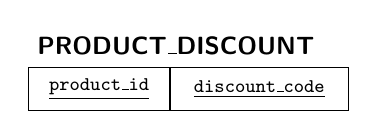
\begin{tikzpicture}[font=\scriptsize\ttfamily, box/.style={draw,minimum height=0.55cm,inner sep=2pt,anchor=west}]
\node[anchor=south west,font=\small\bfseries\sffamily] at (0,0.32) {PRODUCT\_DISCOUNT};
\node[box,minimum width=1.80cm] at (0.00,0) {\underline{product\_id}};
\node[box,minimum width=2.27cm] at (1.80,0) {\underline{discount\_code}};
\end{tikzpicture}
\end{adjustbox}\par\medskip

\par\noindent\begin{adjustbox}{max width=\linewidth}
\begin{tikzpicture}[font=\scriptsize\ttfamily, box/.style={draw,minimum height=0.55cm,inner sep=2pt,anchor=west}]
\node[anchor=south west,font=\small\bfseries\sffamily] at (0,0.32) {RETURN\_ITEM};
\node[box,minimum width=1.49cm] at (0.00,0) {\underline{order\_id}};
\node[box,minimum width=1.33cm] at (1.49,0) {\underline{item\_no}};
\node[box,minimum width=1.80cm] at (2.83,0) {return\_qty};
\node[box,minimum width=2.27cm] at (4.62,0) {refund\_amount};
\node[anchor=east,font=\scriptsize\sffamily\bfseries] at (-0.05,-0.79) {FD1};
\draw (0.74,-0.79) -- (5.76,-0.79);
\draw[line width=1.1pt] (0.74,-0.28) -- (0.74,-0.79);
\draw[line width=1.1pt] (2.16,-0.28) -- (2.16,-0.79);
\draw[-{Stealth[length=4pt]}] (3.73,-0.79) -- (3.73,-0.28);
\draw[-{Stealth[length=4pt]}] (5.76,-0.79) -- (5.76,-0.28);
\end{tikzpicture}
\end{adjustbox}\par\medskip


\subsection{正規化後更新 Schema 的 SQL}

以下為正規化後有變動的部分，完整 SQL 見 4.6 節與 Appendix。

\textbf{ORDERS：}刪除 \at{total}，改以 CHECK 檢查 BR-09 的算式不為負（\at{01_schema.sql}）。
\VerbatimInput[fontsize=\scriptsize,numbers=left,numbersep=4pt,firstline=67,lastline=85]{sql/01_schema.sql}

\textbf{PRODUCT\_DISCOUNT：}只保留兩個外鍵欄位。
\VerbatimInput[fontsize=\scriptsize,numbers=left,numbersep=4pt,firstline=133,lastline=139]{sql/01_schema.sql}

\textbf{RETURN\_ITEM：}以 \at{(order_id, item_no)} 為主鍵，分別參照 \at{RETURN_REQUEST} 與 \at{ORDER_ITEM}。
\VerbatimInput[fontsize=\scriptsize,numbers=left,numbersep=4pt,firstline=164,lastline=172]{sql/01_schema.sql}

\textbf{檢視表 v\_orders：}需要訂單總額時查詢這個檢視表。
\VerbatimInput[fontsize=\scriptsize,numbers=left,numbersep=4pt,firstline=191,lastline=195]{sql/01_schema.sql}

\textbf{BR-13 trigger：}取代原本的 EXCLUDE 限制（\at{02_triggers.sql}）。新增或修改 \at{product_discount} 時，\at{product_discount_check} 先確認折扣是特殊活動折扣，再檢查同一商品已套用的其他特殊活動折扣期間是否重疊；修改 \at{discount} 的期間時，\at{discount_period_check} 對該折扣套用的每項商品重新檢查。檢查前以 \at{pg_advisory_xact_lock} 鎖住該商品，避免兩筆交易同時寫入而都通過檢查。實際被拒絕的例子見 4.8 節圖 \ref{fig:db8}。
\VerbatimInput[fontsize=\scriptsize,numbers=left,numbersep=4pt,firstline=234,lastline=285]{sql/02_triggers.sql}

% ================= Section 6 =================
\clearpage
\section{資料庫系統的使用 (The Use of the Database System)}

\subsection{系統安裝 (System Installation Description)}

系統有兩種使用方式：直接開啟線上版，或在本機以 Docker 安裝。

\textbf{線上版。}系統已部署在 \texttt{https://fuwafuwa-eshop.vercel.app}，打開瀏覽器即可使用，示範帳號與下方相同。前端與 FastAPI 後端部署在 Vercel（後端以 Python serverless function 執行），資料庫使用 Neon 的 PostgreSQL（美國東部 us-east-1），同樣執行 Appendix 的四個 SQL 檔建立。線上版與本機版的程式和資料庫綱要相同。

\textbf{本機安裝。}本機版由三個 Docker 容器組成：PostgreSQL 16 資料庫、FastAPI 後端（Python，JWT 登入、SQLAlchemy 存取資料庫）與 React + Vite 前端。資料庫第一次啟動時，會依檔名順序自動執行 \at{db/init/} 中的四個 SQL 檔（即 Appendix 的 SQL）。

\textbf{安裝需求。}安裝 Docker Desktop 即可，不需要另外安裝 PostgreSQL、Python 或 Node.js。

\textbf{啟動步驟。}在專案根目錄執行：
\begin{Verbatim}[fontsize=\small,xleftmargin=2em]
./start.sh            # 等同 docker compose up --build
./start.sh reset      # 清空資料庫，重新執行 db/init/*.sql
./start.sh down       # 停止所有容器
\end{Verbatim}

\begingroup\small
\begin{xltabular}{\linewidth}{|>{\raggedright\arraybackslash}p{4cm}|>{\raggedright\arraybackslash}X|}
\caption{系統服務與網址}\\
\hline\rowcolor{headgray}\textbf{服務} & \textbf{網址}\\\hline\endhead
網站（三種介面） & \texttt{http://localhost:5173}\\\hline
後端 API 文件（Swagger） & \texttt{http://localhost:8001/docs}\\\hline
PostgreSQL & \texttt{localhost:5433}，帳號、密碼、資料庫名稱皆為 \texttt{fuwa}\\\hline
\end{xltabular}
\endgroup

\textbf{示範帳號。}\at{03_seed.sql} 建立了以下帳號，登入後依角色進入不同的介面：

\begingroup\small
\begin{xltabular}{\linewidth}{|>{\raggedright\arraybackslash}p{2cm}|>{\raggedright\arraybackslash}p{2.4cm}|>{\raggedright\arraybackslash}p{3.4cm}|>{\raggedright\arraybackslash}X|}
\caption{示範帳號}\\
\hline\rowcolor{headgray}\textbf{帳號} & \textbf{密碼} & \textbf{角色} & \textbf{進入的介面}\\\hline\endhead
\texttt{admin} & \texttt{admin123} & 平台管理員 & 平台管理介面（\texttt{/admin}）\\\hline
\texttt{staff} & \texttt{staff123} & 工作人員 & 工作人員管理介面（\texttt{/staff}）\\\hline
\texttt{manager} & \texttt{staff123} & 工作人員、平台管理員 & 兩個介面都能進入，頁首可切換\\\hline
\texttt{alice}、\texttt{bob} & \texttt{customer123} & 顧客 & 顧客購物介面\\\hline
\texttt{carol} & \texttt{customer123} & 顧客（已停用） & 無法登入，用來示範停用帳號\\\hline
\end{xltabular}
\endgroup


\subsection{系統使用 (The Use of the System)}

\newcommand{\guishot}[2]{% {檔名}{說明}
\begin{figure}[htbp]\centering\includegraphics[width=0.92\linewidth]{img/#1}\caption{#2}\end{figure}}

同一個網站依登入者的角色顯示三種介面：顧客購物介面、工作人員管理介面與平台管理介面。以下截圖為系統以 4.7 節的示範資料啟動後實際操作的畫面。

\subsubsection*{顧客購物介面}

未登入的訪客也可以瀏覽商品。首頁（圖 \ref{fig:gui_home}）上方列出今天有效的折扣政策，可以依關鍵字、商店與類別搜尋商品；點選商品進入商品頁（圖 \ref{fig:gui_product}）。商店一覽（圖 \ref{fig:gui_stores}）列出三間商店與其平均評分。

\guishot{gui_home.png}{\label{fig:gui_home}首頁：今日優惠、商品搜尋與篩選}
\guishot{gui_product.png}{\label{fig:gui_product}商品頁}
\guishot{gui_stores.png}{\label{fig:gui_stores}商店一覽與評分}

登入頁（圖 \ref{fig:gui_login}）以帳號與密碼登入，已停用的帳號無法登入。顧客登入後可以把商品加入購物車並調整數量（圖 \ref{fig:gui_cart}），結帳後在「我的訂單」查看所有訂單與消費總額（圖 \ref{fig:gui_my_orders}）；訂單詳情顯示訂單進度與狀態歷程（圖 \ref{fig:gui_order_detail}），狀態歷程即 \at{order_status_history} 中由 trigger 寫入的資料。

\guishot{gui_login.png}{\label{fig:gui_login}登入頁}
\guishot{gui_cart.png}{\label{fig:gui_cart}購物車（顧客 alice）}
\guishot{gui_my_orders.png}{\label{fig:gui_my_orders}我的訂單}
\guishot{gui_order_detail.png}{\label{fig:gui_order_detail}訂單詳情與狀態歷程（訂單 \#5）}

\subsubsection*{工作人員管理介面}

工作人員登入後進入後台總覽（圖 \ref{fig:gui_staff_dashboard}），顯示期間內的訂單數、銷售總額、各狀態的訂單數與待審核的退貨。商品與庫存（圖 \ref{fig:gui_staff_products}）可以新增、修改、上下架與刪除商品；已被訂單引用的商品刪除時會改為下架（BR-20）。

\guishot{gui_staff_dashboard.png}{\label{fig:gui_staff_dashboard}工作人員後台總覽}
\guishot{gui_staff_products.png}{\label{fig:gui_staff_products}商品與庫存管理}

隸屬商店的工作人員只能管理自己商店的資料（BR-21）。圖 \ref{fig:gui_store_staff_products} 是台北信義店店員 \texttt{staff\_xinyi} 登入後的商品頁，商店篩選固定為自己的商店，只列出該店的 5 項商品；訂單、退貨與報表也只顯示含該店商品的資料。

\guishot{gui_store_staff_products.png}{\label{fig:gui_store_staff_products}商店工作人員只看得到自己商店的商品}

訂單管理（圖 \ref{fig:gui_staff_orders}）可以依狀態、日期與關鍵字查詢訂單；在訂單詳情（圖 \ref{fig:gui_staff_order_detail}）依 BR-19 的順序推進狀態。圖中訂單 \#10 有待審核的退貨申請，因此依 BR-25 不能推進狀態，畫面上方顯示提示。

\guishot{gui_staff_orders.png}{\label{fig:gui_staff_orders}訂單管理}
\guishot{gui_staff_order_detail.png}{\label{fig:gui_staff_order_detail}訂單詳情：有待審核退貨時不能推進狀態（BR-25）}

退貨審核（圖 \ref{fig:gui_staff_returns}）列出所有退貨申請，核准時依 BR-26 計算退款金額。折扣管理（圖 \ref{fig:gui_staff_discounts}）管理特殊活動、季節性與運費三種折扣，特殊活動折扣可以指定適用商品，期間重疊時會被 5.4 節的 BR-13 trigger 拒絕。銷售報表（圖 \ref{fig:gui_staff_reports}）依日、週、月統計各商店的銷售額，計算方式與 Section 8 的檢視表 V1 相同（BR-23）。

\guishot{gui_staff_returns.png}{\label{fig:gui_staff_returns}退貨審核}
\guishot{gui_staff_discounts.png}{\label{fig:gui_staff_discounts}折扣管理}
\guishot{gui_staff_reports.png}{\label{fig:gui_staff_reports}銷售報表}

\subsubsection*{平台管理介面}

平台管理員可以查詢、新增與修改使用者帳號，指派角色、指定工作人員所屬的商店（未指定即為總部人員，AAS-F-009），以及停用或啟用任何帳號（圖 \ref{fig:gui_admin_users}）；系統至少保留一位啟用中的平台管理員。商店資料（圖 \ref{fig:gui_admin_stores}）用來新增商店（STS-F-005）與修改各商店的聯絡資訊（STS-F-002）。

\guishot{gui_admin_users.png}{\label{fig:gui_admin_users}使用者帳號、角色與停用／啟用}
\guishot{gui_admin_stores.png}{\label{fig:gui_admin_stores}商店資料}

\subsubsection*{手機版}

網站採用響應式版面，在手機寬度下導覽列收成選單按鈕，商品列表改為兩欄，後台側欄也會收合（圖 \ref{fig:gui_mobile}）。

\begin{figure}[htbp]\centering
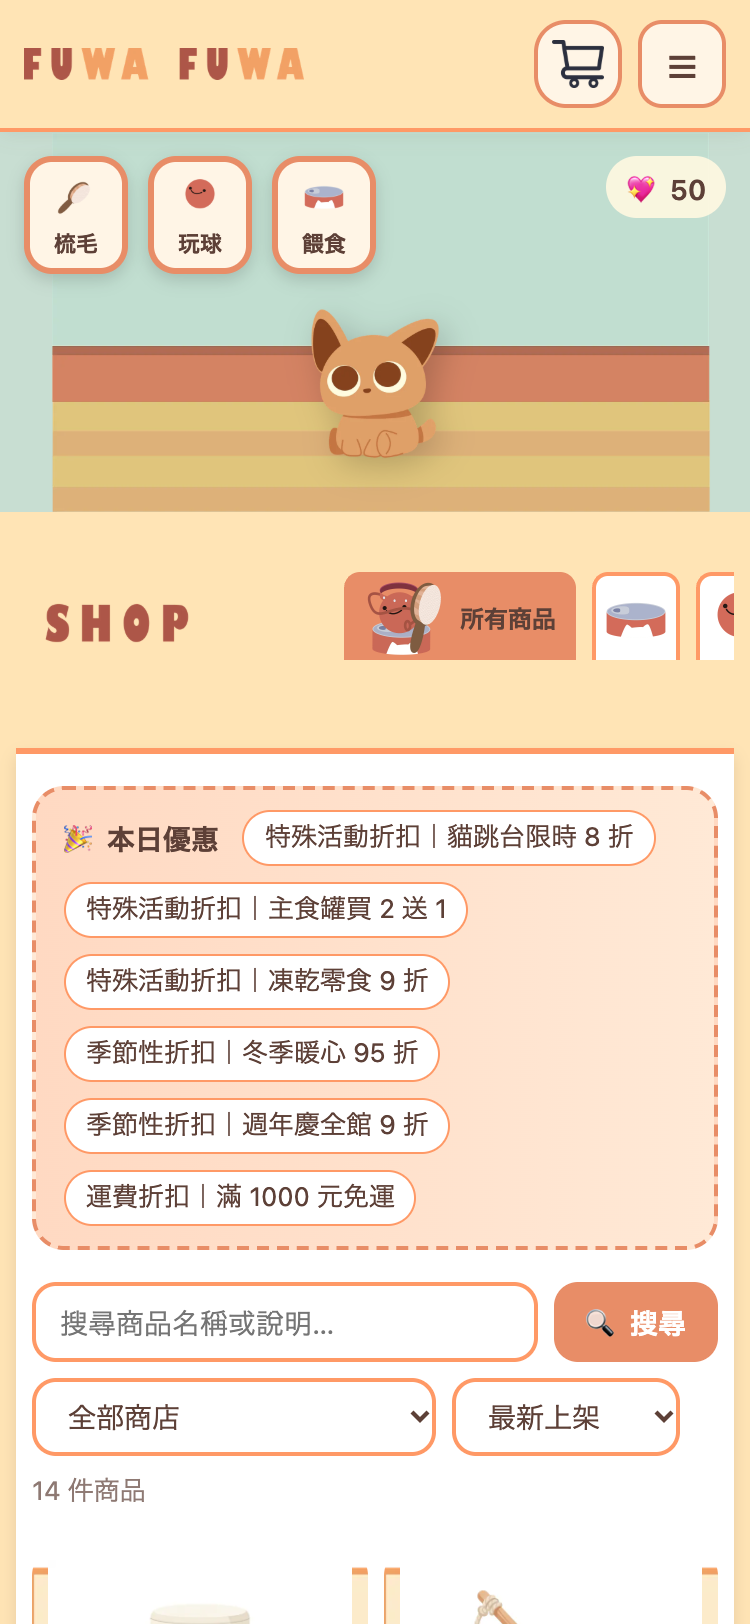
\includegraphics[width=0.36\linewidth]{img/gui_mobile_home.png}\hspace{2em}%
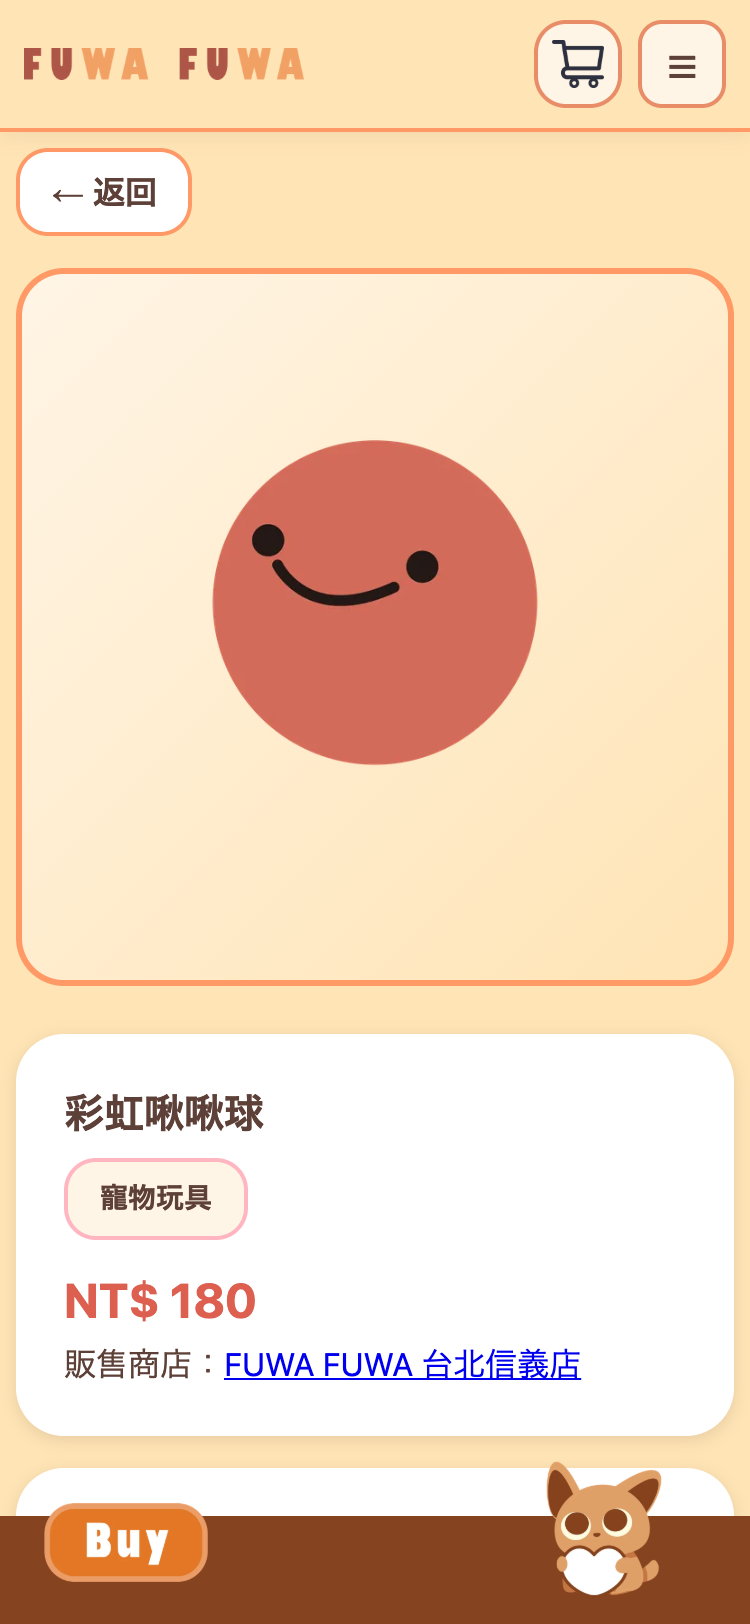
\includegraphics[width=0.36\linewidth]{img/gui_mobile_product.png}
\caption{\label{fig:gui_mobile}手機版（375 像素寬）的首頁與商品頁}
\end{figure}


% ================= Section 7 =================
\clearpage
\section{資料庫調校建議 (Suggestions of Database Tuning)}

\subsection{索引結構 (Index Structures)}

PostgreSQL 會自動替主鍵與 UNIQUE 建立 B-tree 索引，但\textbf{不會}自動替外鍵建立索引。依 4.4 節的操作頻率，下列查詢最常執行，建議加上索引：

\begingroup\small
\begin{xltabular}{\linewidth}{|>{\raggedright\arraybackslash}p{5.6cm}|>{\raggedright\arraybackslash}X|}
\caption{建議的索引}\\
\hline\rowcolor{headgray}\textbf{索引} & \textbf{用途}\\\hline\endhead
\at{CREATE EXTENSION pg_trgm;} \at{CREATE INDEX ON product USING gin (name gin_trgm_ops, description gin_trgm_ops);} & 關鍵字搜尋（PMS-F-001）是讀取量最大的操作，\texttt{ILIKE '\%關鍵字\%'} 無法使用 B-tree，trigram GIN 索引可以避免掃描整張商品表\\\hline
\at{CREATE INDEX ON product (store_id) WHERE is_listed;} & 商店頁列出該店上架中的商品（STS-F-001）\\\hline
\at{CREATE INDEX ON orders (user_id, order_time DESC);} & 顧客查詢自己的歷史訂單並依時間排序（OMS-F-005）\\\hline
\at{CREATE INDEX ON orders (status, order_time);} & 工作人員依狀態與日期篩選訂單（OMS-F-006）\\\hline
\at{CREATE INDEX ON orders (paid_at);} & 日、週、月報表依付款日期範圍查詢（RSS-F-001～003）\\\hline
\at{CREATE INDEX ON order_item (product_id);} & 暢銷商品統計、商品被訂單引用時改為下架的檢查（PMS-F-007）\\\hline
\at{CREATE INDEX ON product_discount (discount_code);} & 依折扣查詢適用商品、修改折扣期間時的 BR-13 檢查\\\hline
\at{CREATE INDEX ON order_discount (discount_code);} & 折扣是否被訂單使用過的檢查（DMS-F-007）、Q4 統計\\\hline
\at{CREATE INDEX ON return_request (order_id) WHERE status = 'pending';} & 更新訂單狀態前檢查是否有待審核的退貨（BR-25），部分索引只包含少量 pending 資料\\\hline
\at{CREATE INDEX ON store_review (store_id);} & 商店頁顯示平均評分與評論列表（STS-F-004）\\\hline
\end{xltabular}
\endgroup

\textbf{實測：加索引前後的比較。}示範資料只有 15 項商品、13 筆訂單，看不出索引的差別，因此我們另外啟動一個測試用資料庫，以 \at{sql_bench/bench_data.sql} 產生\textbf{測試資料}：依 4.5 節估計的一年訂單量，產生 20,000 位顧客、109,500 筆訂單與約 33 萬筆訂單明細，並把商品數放大到 10 萬項，其中約 0.2\% 的商品名稱含有「貓抓板」。這些資料只用來量測效能，不是真實資料，也沒有放進正式的資料庫。測試的兩個查詢是讀取量最大的商品關鍵字搜尋，以及顧客查詢自己的歷史訂單（4.4 節）。為了讓執行計畫簡短，關鍵字搜尋只比對商品名稱，所以 trigram 索引也只建在 \at{name} 上。

\resultimg{bench_before.png}{加索引前：兩個查詢都要循序掃描整張表（Seq Scan）}
\resultimg{bench_index.png}{建立 trigram GIN 索引與 \at{(user_id, order_time DESC)} 索引}
\resultimg{bench_after.png}{加索引後：兩個查詢都改用索引（Bitmap Index Scan）}

\begingroup\small
\begin{xltabular}{\linewidth}{|>{\raggedright\arraybackslash}X|>{\raggedleft\arraybackslash}p{2.2cm}|>{\raggedleft\arraybackslash}p{2.2cm}|>{\raggedleft\arraybackslash}p{1.6cm}|}
\caption{加索引前後的執行時間（\at{EXPLAIN ANALYZE} 的 Execution Time，連續執行 6 次、捨去第 1 次後取中位數）}\\
\hline\rowcolor{headgray}\textbf{查詢} & \textbf{加索引前} & \textbf{加索引後} & \textbf{加速}\\\hline\endhead
商品關鍵字搜尋（10 萬項商品中找出 194 項） & 27.18 ms & 0.46 ms & 約 59 倍\\\hline
顧客的歷史訂單（109,513 筆訂單中找出 4 筆） & 4.54 ms & 0.07 ms & 約 63 倍\\\hline
\end{xltabular}
\endgroup

加索引前，PostgreSQL 必須讀過整張表再逐筆過濾，例如歷史訂單查詢為了找出 4 筆訂單，丟掉了其餘 109,509 筆；加索引後只讀取符合條件的資料，兩個查詢都快了約 60 倍。資料量越大，循序掃描的時間會跟著線性增加，用索引查詢的時間則幾乎不變，所以這兩個索引的效益會隨營運時間持續擴大。重新產生截圖的指令為 \at{tools/make_bench_shots.sh}。

\subsection{資料庫設計 (Database Design)}

\begin{itemize}[itemsep=0.3em]
  \item \textbf{報表改用 materialized view。}V1 的銷售報表需要彙總所有訂單明細，資料量隨時間線性成長（4.5 節），但過去日期的報表不會再變動。可以把 V1 建成 materialized view，每天凌晨 \at{REFRESH MATERIALIZED VIEW CONCURRENTLY} 一次，工作人員查詢報表時就不必每次重新計算。
  \item \textbf{歷史資料分割。}\at{orders}、\at{order_item}、\at{order_status_history} 是成長最快的三張表，資料量變大後可以依 \at{order_time} 做 range partition（例如每年一個分割），查詢近期訂單時只需掃描最新的分割。
  \item \textbf{購物車清理。}長期沒有結帳的 \at{cart_item} 可以定期清除，避免購物車資料無限累積。
\end{itemize}

\subsection{查詢 (Queries)}

\begin{itemize}[itemsep=0.3em]
  \item \textbf{結帳時依固定順序鎖定商品。}結帳交易以 \at{SELECT … FOR UPDATE} 鎖定購物車中的商品再扣庫存（BR-06）；鎖定時依 \at{product_id} 排序，可避免兩位顧客同時結帳時互相等待而發生 deadlock。
  \item \textbf{只查需要的欄位。}商品列表不需要 \at{description} 這類長文字，只查列表需要的欄位可以減少傳輸量。
  \item \textbf{避免 N+1 查詢。}顯示訂單列表時以 JOIN 或一次 \at{IN (…)} 查出所有明細，而不是每筆訂單各查一次。
\end{itemize}

\subsection{系統部署後的效能改善}

系統部署到線上（6.1 節）後，另外做了三項不涉及資料庫綱要的改善：
\begin{itemize}[itemsep=0.3em]
  \item \textbf{批次查詢折扣，去掉 N+1 查詢。}商品列表原本對每項商品各查一次是否有進行中的特殊活動折扣，列出 $n$ 項商品就要 $n+1$ 次查詢；改為以 \at{product_id IN (…)} 一次查出所有商品的折扣。
  \item \textbf{圖片改用 WebP。}網站圖片縮小尺寸並轉成 WebP，總大小由約 12~MB 降到約 0.3~MB；\at{product.image_url} 也改指向 \at{.webp} 檔（\at{03_seed.sql}）。
  \item \textbf{CDN 快取。}前端打包的靜態檔快取一年、圖片快取一天；未登入時查詢商品、商店與進行中折扣的回應設定 \at{s-maxage=30}，讓 CDN 最多快取 30 秒；實測連續查詢 \at{/api/stores/}，第一次為 \at{x-vercel-cache: MISS}，30 秒內的後續查詢為 \at{HIT}，由 CDN 直接回應、不再查詢資料庫。登入後的請求一律不快取，庫存與價格仍在加入購物車與結帳時由資料庫即時檢查（BR-05、BR-06）。
\end{itemize}


% ================= Section 8 =================
\clearpage
\section{額外的查詢與檢視表 (Additional Queries and Views)}

本節實作 2 個檢視表與 4 個查詢，涵蓋聚合函數（COUNT、SUM、AVG、MAX）、GROUP BY、HAVING、ORDER BY 與巢狀查詢，對應報表統計子系統（RSS）與商店、折扣的管理需求。SQL 檔位於 \at{phase4/sql_q/}。正規化後 \at{orders} 不再儲存總額，需要訂單總額的 V1、Q2 改查檢視表 \at{v_orders}（5.3 節）。以下結果為在 PostgreSQL 16 上對示範資料執行的截圖。

\begingroup\small
\begin{xltabular}{\linewidth}{|>{\raggedright\arraybackslash}p{3.8cm}|>{\centering\arraybackslash}p{1.3cm}|>{\centering\arraybackslash}p{1.4cm}|>{\centering\arraybackslash}p{1.4cm}|>{\centering\arraybackslash}p{1.4cm}|X|}
\caption{各查詢與檢視表使用的 SQL 功能}\\
\hline\rowcolor{headgray}\textbf{查詢／檢視表} & \textbf{聚合} & \textbf{GROUP BY} & \textbf{ORDER BY} & \textbf{巢狀查詢} & \textbf{其他}\\\hline\endhead
V1 \at{v_store_daily_sales} & $\surd$ & $\surd$ & $\surd$ & $\surd$ & CTE、window function\\\hline
V2 \at{v_product_sales} & $\surd$ & $\surd$ & $\surd$ & & 四表 JOIN\\\hline
Q1 各店銷售冠軍 & $\surd$ & & $\surd$ & $\surd$ & 相關子查詢\\\hline
Q2 高消費顧客 & $\surd$ & $\surd$ & $\surd$ & $\surd$ & HAVING\\\hline
Q3 商店評分 & $\surd$ & $\surd$ & $\surd$ & $\surd$ & LEFT JOIN\\\hline
Q4 折扣使用統計 & $\surd$ & $\surd$ & $\surd$ & & LEFT JOIN\\\hline
\end{xltabular}
\endgroup

\subsection{檢視表 V1：各商店每日銷售報表}
對應 RSS-F-001 與 BR-23。一筆訂單可以包含多間商店的商品，因此先算出每間商店的商品在該訂單中扣除特殊活動折扣後的金額（\at{share}），再依比例分攤訂單總額；部分退貨的訂單從該商店扣除退款金額，已取消或全部退貨的訂單不計入。週報與月報只要把 \at{sales_date} 換成 \at{date_trunc('week', …)} 或 \at{date_trunc('month', …)} 再加總即可。
\VerbatimInput[fontsize=\scriptsize,numbers=left,numbersep=4pt]{sql_q/v1_store_daily_sales.sql}
\resultimg{q_v1.png}{V1 執行結果}

\subsection{檢視表 V2：各商品銷售統計}
對應 RSS-F-004（暢銷商品）。彙總每項商品的訂單數、銷售數量與扣除特殊活動折扣後的營收。
\VerbatimInput[fontsize=\scriptsize,numbers=left,numbersep=4pt]{sql_q/v2_product_sales.sql}
\resultimg{q_v2.png}{V2 執行結果（銷售量前 10 名）}

\subsection{查詢 Q1：每間商店的銷售冠軍商品}
以相關子查詢找出每間商店銷售量等於該店最大值的商品。
\VerbatimInput[fontsize=\scriptsize,numbers=left,numbersep=4pt]{sql_q/q1_store_best_seller.sql}
\resultimg{q_q1.png}{Q1 執行結果}

\subsection{查詢 Q2：消費總額高於平均的顧客}
內層子查詢先算出每位顧客的消費總額再取平均，外層以 HAVING 篩選高於平均的顧客，依消費金額由高到低排序。
\VerbatimInput[fontsize=\scriptsize,numbers=left,numbersep=4pt]{sql_q/q2_top_customers.sql}
\resultimg{q_q2.png}{Q2 執行結果}

\subsection{查詢 Q3：各商店的平均評分}
對應 STS-F-004。用 LEFT JOIN 讓沒有評價的商店也列出，並以純量子查詢計算上架中的商品數。
\VerbatimInput[fontsize=\scriptsize,numbers=left,numbersep=4pt]{sql_q/q3_store_rating.sql}
\resultimg{q_q3.png}{Q3 執行結果}

\subsection{查詢 Q4：各折扣政策的使用統計}
列出每個折扣政策被多少筆訂單使用、總共折抵多少金額，從未使用的折扣也會列出，方便工作人員評估促銷效果。
\VerbatimInput[fontsize=\scriptsize,numbers=left,numbersep=4pt]{sql_q/q4_discount_usage.sql}
\resultimg{q_q4.png}{Q4 執行結果}


% ================= Section 9 =================
\clearpage
\section{結論與未來工作 (Conclusions and Future Work)}

\subsection{結論}

本專題依 Phase 1 的需求分析、Phase 2 的 ER Model 與 Schema，在 PostgreSQL 上實作了 FUWA FUWA e-Shop 的資料庫與網站。資料庫以主鍵、外鍵、UNIQUE、CHECK 與 trigger 實作 26 條商業規則中與資料有關的限制，因此即使繞過網站直接操作資料庫，不合法的資料也會被拒絕。Phase 4 分析各資料表的函數相依並正規化，讓重複的資料只存一份，原本靠重複欄位實作的限制改由 trigger 檢查。

\subsection{未來工作}

\begin{itemize}[itemsep=0.2em]
  \item 各商店獨立管理權限：目前工作人員可以管理所有商店，未來可讓工作人員只管理自己所屬商店的商品、訂單與報表。
  \item 串接第三方金流與物流，實際完成付款與退款。
  \item 商品搜尋改用全文檢索，並加入推薦功能（PMS-F-008）。
\end{itemize}

\subsection{組員心得與分工}

\todo{每位組員各自撰寫負責的工作與心得（徐法恩、魏提安、鄧玉璿、黃柏瑋、陳俊佑）。}
